\documentclass[10pt]{beamer}


\usepackage{graphicx} % Pour les images


\usetheme[progressbar=frametitle]{metropolis}
\usepackage{appendixnumberbeamer}
\usepackage{booktabs}
\usepackage[scale=2]{ccicons}
\usepackage{pgfplots}
\usepgfplotslibrary{dateplot}
\usepackage{xspace}
\usepackage{tikz} % Pour les flèches et les diagrammes
\usepackage{array} % Pour les tableaux
\usepackage{eurosym}
\usepackage{enumitem}
\usepackage{tikz}
\usepackage{fontenc}
\usepackage{ulem}

\setbeamercolor{background canvas}{bg=white}


% Redéfinir la commande \insertframenumber pour inclure le logo
\addtobeamertemplate{frametitle}{}{
  \tikz[remember picture,overlay] 
    \node[anchor=north east,inner sep=0cm] at (current page.north east) {
      
\includegraphics[height=0.97cm]{images/logo.png}
    };
}
% Définir les styles par défaut
\setlist[itemize,1]{label=\textbullet} % Premier niveau : point plein
\setlist[itemize,3]{label=\textendash} % Deuxième niveau : tiret long
\setlist[itemize,2]{label=$\circ$} % Troisième niveau : cercle vide

% Définir les styles par défaut pour enumerate
\setlist[enumerate,1]{label=\arabic*.} % Premier niveau : chiffres arabes
\setlist[enumerate,2]{label=\Alph*.} % Deuxième niveau : lettres majuscules
\setlist[enumerate,3]{label=\alph*.} % Troisième niveau : lettres minuscules

% Logo à gauche et à droite
\titlegraphic{
  
\includegraphics[height=1.3cm]{images/logo_univ.png}\hfill
  
\includegraphics[height=1.3cm]{images/logo_CMI.png}\\[3cm] % Espace entre les logos du haut et le logo Cibest
  \vspace{0.1cm} % Ajoute un espace vertical pour descendre le logo Cibest plus bas
  \hfill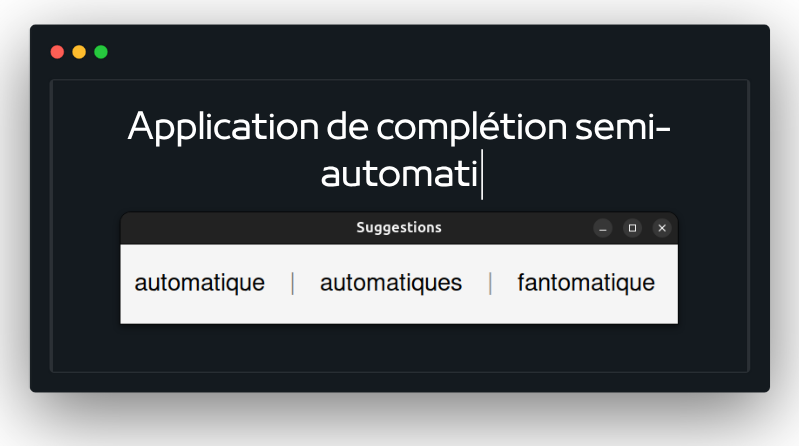
\includegraphics[height=3.1cm]{images/illustration_borderless.png}
}



\title{\vspace{1cm}Complétion semi-automatique\\Projet d'Initiation à la recherche}
\author{Samia Benali \& Elouan BOITEUX\\[0.3cm]Année universitaire 2024 -- 2025 \\[0.3cm]CMI Informatique Deuxième Année\\[0.3cm] Référent : Pierre-Cyril HEAM \\[0.3cm]22 mai 2025}
\date{}



\begin{document}

\maketitle

\begin{frame}{Table des matières}
	\setbeamertemplate{section in toc}[sections numbered]
	\tableofcontents%[hideallsubsections]
\end{frame}


\section{La complétion semi-automatique}

\begin{frame}{Définition complétion semi-automatique}
	\begin{columns}
		\column{0.45\textwidth}
		
		\textbf{En quelques mots~:}
		\begin{itemize}
			\item Assistance
			\item Proposition des suggestions
			\item Choix final fait par l'utilisateur
		\end{itemize}
		\vfill	
		\textbf{Utilisé dans de nombreuses applications~:}
		\begin{itemize}
			\item Traitement de texte
			\item IDE
			\item Moteurs de recherche
			\item Assistance virtuelle
		\end{itemize}
		\column{0.55\textwidth}
		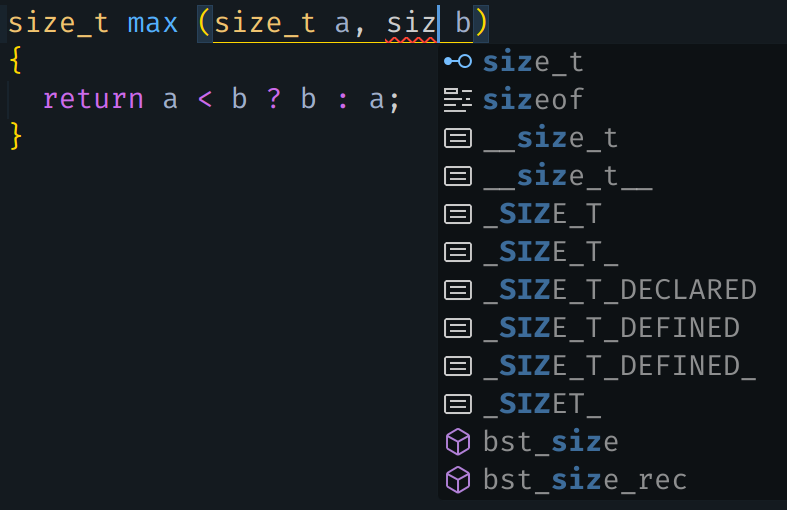
\includegraphics[width=\textwidth]{images/exemple_completion_semi_auto.png}
            \centering
		\uline{Exemple de complétion semi-automatique sur VS Code}
		
	\end{columns}
\end{frame}


\begin{frame}{Différence avec la complétion semi-automatique}
	\begin{columns}
		\column{0.48\textwidth}
		\textbf{Automatique}
		\begin{itemize}
			\item Pas besoin d'interactions manuelles
			\item Génération d'erreurs si le contexte est mal interprété
		\end{itemize}
		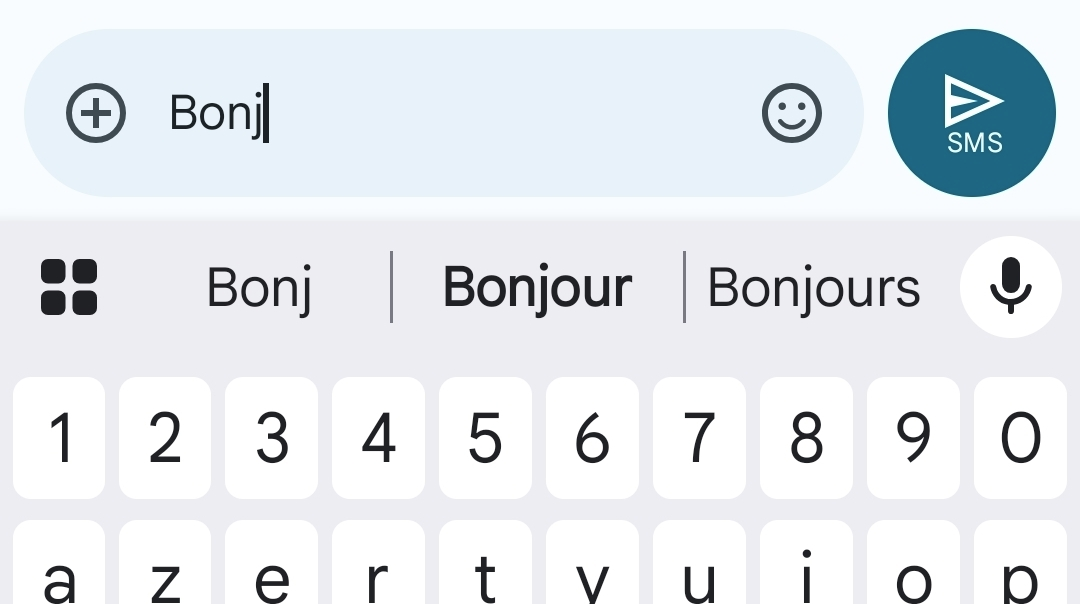
\includegraphics[width=0.9\textwidth]{images/exemple_clavier_completion_auto.png}
		
		\column{0.48\textwidth}
		\textbf{Semi-Automatique}
		\begin{itemize}
			\item Nécessite une validation manuelle
			\item Plus de contrôle pour l'utilisateur
			\item Moins d’erreurs
		\end{itemize}
		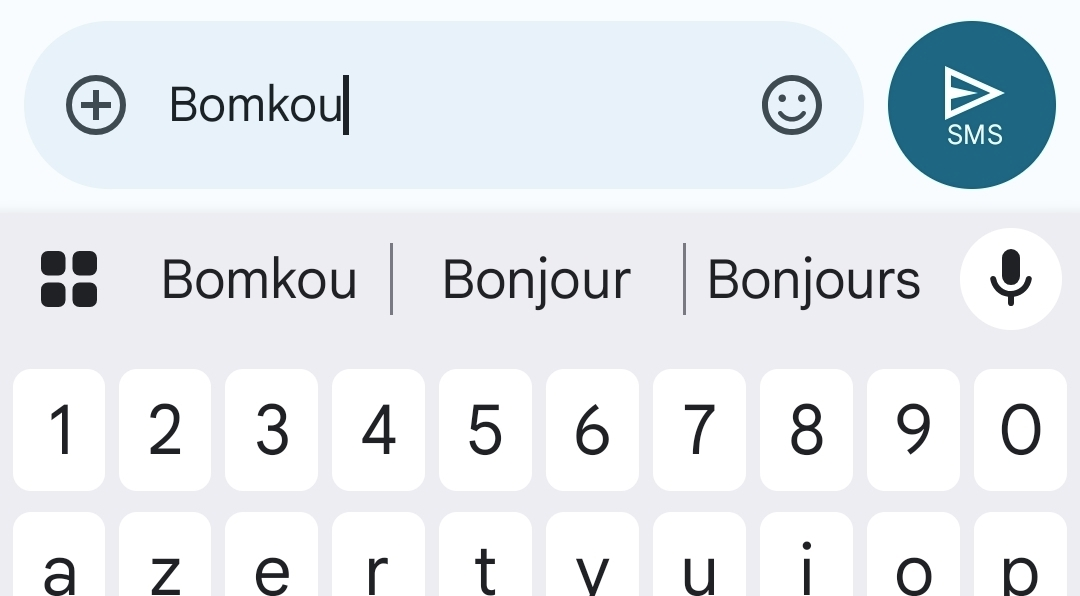
\includegraphics[width=0.9\textwidth]{images/exemple_clavier_completion_semi.png}
	\end{columns}
\end{frame}

% \begin{frame}{Cibest}
%     \begin{columns}[T]
%         \metroset{block=fill}
%         \column{0.45\textwidth}
%         \begin{exampleblock}{Cibest Solution}
%                 \textbf{Champs d'action~:}
%                 \begin{itemize}
%                     \item Domaine du logiciel\\embarqué
%                     \item Vidéoprotection
%                     \item Wifi passagers
%                     \item Comptage passagers
%                     \item Rétrovision numérique
%                 \end{itemize}

%                 \textbf{Statistiques~:}
%                 \begin{itemize}
%                     \item + de 450 clients équipés
%                     \item + de 200 villes en France
%                 \end{itemize}
%           \end{exampleblock}

%         \column{0.45\textwidth}
%         \begin{alertblock}{Cibest IT}
%             \textbf{Champs d'action~:}
%             \begin{itemize}
%                 \item Informatique dans les\\transports
%                 \item Billetique
%             \end{itemize}

%             \textbf{Statistiques~:}
%             \begin{itemize}
%                 \item + de 30 consultants clients équipés
%                 \item + de 200 villes en France
%             \end{itemize}
%           \end{alertblock}
%     \end{columns}
%     \end{frame}


%
% \section{Missions du Stage}
% \begin{frame}{Contexte et Problématique Actuelle}
% 	\begin{columns}
% 		\column{0.5\textwidth}
% 		\textbf{Contexte}
% 		\begin{itemize}
% 			\item Installation d'équipements
% 			\item Configurations personnalisées
% 			\item Sauvegarde des configurations
% 			\item Identification des problèmes
% 		\end{itemize}
% 		
% 		\column{0.5\textwidth}
% 		\textbf{Problématique}
% 		\begin{itemize}
% 			\item Récupération manuelle
% 			\item Perte de temps, erreurs
% 			\item Résultats sous diverses formes
% 			\item Absence de contrôle qualité
% 		\end{itemize}
% 	\end{columns}
% 	\vfill
% 	\centering\includegraphics[width=0.9\textwidth]{images/camera_bus.png}
% \end{frame}
%
% % Diapositive 2 : Besoins et Solution Proposée
% \begin{frame}{Besoins Identifiés et Solution Proposée}
% 	\begin{columns}
% 		\column{0.7\textwidth}
% 		\hspace*{-0.1\textwidth}
% 		\includegraphics[width=1.1\textwidth]{images/besoins_stage.pdf}
% 		\column{0.3\textwidth}
% 		\hspace*{-0.23\textwidth}
% 		\includegraphics[width=1.4\textwidth]{images/solution_stage.pdf}
% 	\end{columns}
% \end{frame}
% % Diapositive 2 : Besoins et Solution Proposée
% \begin{frame}{Besoins Identifiés et Solution Proposée}
% 	\begin{columns}
% 		\column{0.3\textwidth}
% 		\hspace*{-0.13\textwidth}
% 		\includegraphics[width=1.2\textwidth]{images/besoins_stage.pdf}
% 		
% 		\column{0.8\textwidth}
% 		
% 		\hspace*{-0.75cm}
% 		\includegraphics[width=1.125\textwidth]{images/solution_stage.pdf}
% 		
% 	\end{columns}
% \end{frame}
%
%
% \begin{frame}{Méthodologie de Travail}
% 	\begin{columns}[t]
% 		\column{0.5\textwidth}
% 		\textbf{Méthode Agile~:}\\[0.4cm]
% 		\hspace*{-0.4cm}
% 		\vspace*{-1cm}
% 		\begin{itemize}
% 			\item flexibilité
% 			\item adaptabilité
% 			\item amélioration continue
% 		\end{itemize}
% 		\includegraphics[width=1.1\textwidth]{images/schema_conception.png}
% 		\column{0.5\textwidth}
% 		\textbf{Outils Utilisés~:}
% 		\hspace*{0.2cm}
% 		\includegraphics[width=0.8\textwidth]{images/logo_outils.png}
% 	\end{columns}
% \end{frame}

\section{Les différentes approches utilisées}
\begin{frame}{Modèle s'appuyant sur des règles}
	\begin{itemize}
		\item Utilisation d'algorithmes simples s'appuyant sur des règles prédéfinies (correspondance des préfixes et/ou motifs)
		\item Gérer grâce à des dictionnaires statiques ou des listes.
		\item Avantages~: Simplicité et rapidité de mise en œuvre
		\item Inconvénients~: Rigidité, difficulté à gérer des cas complexes
	\end{itemize}
	\begin{center}
		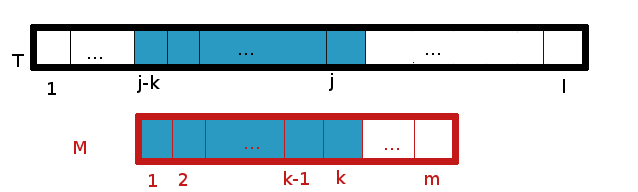
\includegraphics[width=\textwidth]{images/regles.png}
	\end{center}
\end{frame}

\begin{frame}{Modèle s'appuyant sur des statistiques}
	\begin{itemize}
		\item Utilisation de statistiques fournies grâce aux données d'un historique
		\item Prédire des séquence (Markov, TF-IDF)
		\item Avantages~: Résultats rapides et meilleure gestion des cas complexes.
		\item Inconvénients~: Pas de compréhension sémantique et besoin d'un grand nombre de données.
	\end{itemize}
	\begin{center}
		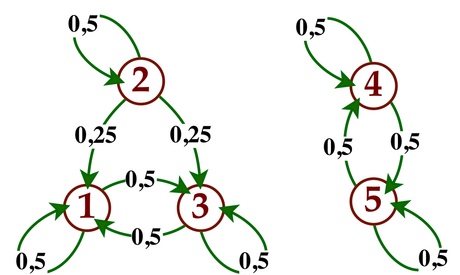
\includegraphics[width=0.5\textwidth]{images/statistiques.png}
	\end{center}
\end{frame}


\begin{frame}{Modèle s'appuyant sur l'intelligence artificielle}
	\begin{columns}
		\column{0.6\textwidth}
		\begin{itemize}
			\item Utilisation d'algorithmes s'appuyant sur l'intelligence artificielle et les réseaux neuronaux
			\item Apprentissage de motifs complexes à partir de données (forêt aléatoires, régressions pour plus de contexte)
			\item Avantages~: Efficace face à des cas complexes et des demandes rares, adaptabilité
			\item Inconvénients~: Nécessite beaucoup de temps de calcul et de ressources
		\end{itemize}
		\column{0.4\textwidth}
		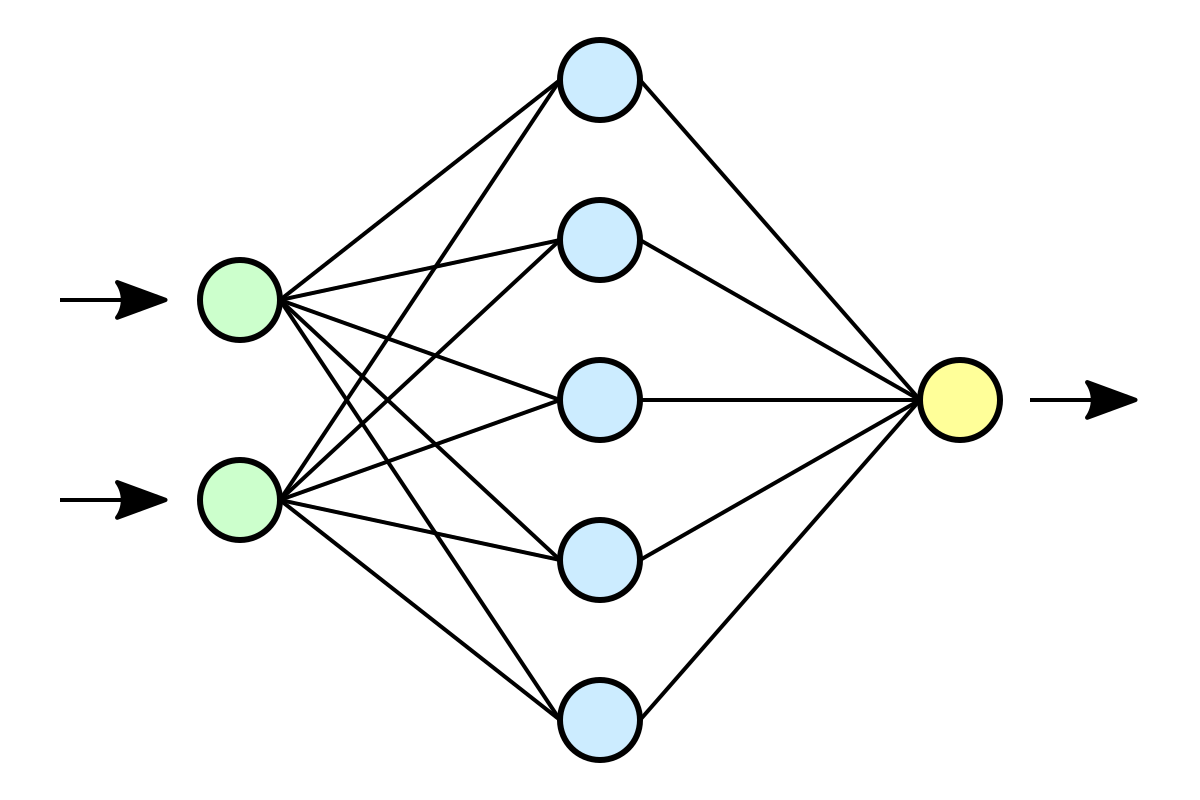
\includegraphics[width=\textwidth]{images/intelligence.png}
	\end{columns}
\end{frame}


\begin{frame}{Modèle s'appuyant sur l'amélioration continue}
	\begin{itemize}
		\item Utilisation d'algorithmes s'appuyant sur l'amélioration en temps réel.
		\item Choix fait par l'utilisateur, choix mémorisés pour une utilisation personnalisée
		\item Avantages~: Implémentation adaptable et avec des suggestions qui ont un sens sémantique, performance très élevée.
		\item Inconvénients~: Implémentation très complexes et longue à déployer, dépend des données collectées et des utilisateurs.
	\end{itemize}
	\begin{center}
		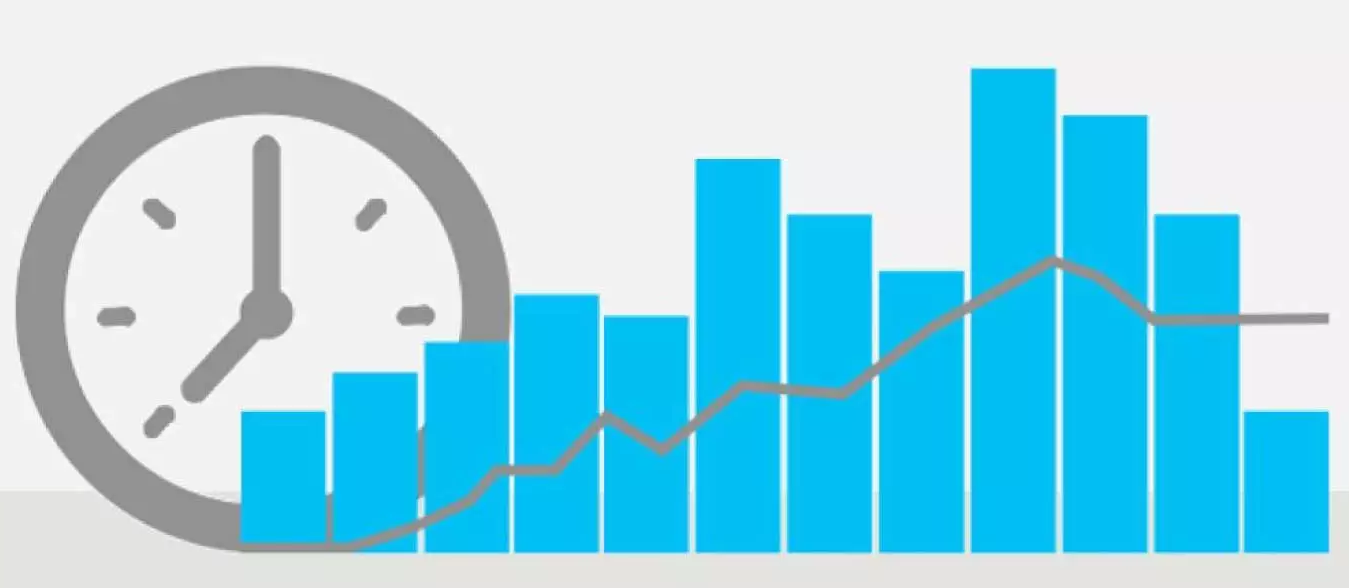
\includegraphics[width=0.6\textwidth]{images/learning.png}
	\end{center}
\end{frame}

\section{Les algorithmes de calcul de distance}
% Un algorithme de calcul de distance permet de mesurer la similarité et/ou la dif-
% férence entre deux objets tels que du texte, des vecteurs, des chaînes de caractères.
% On utilise ces algorithmes de calcul principalement pour la correction d’orthographe,
% le traitement de texte, les alignements de séquences ADN ou encore pour la recherche
% d’information


\begin{frame}{Distance de Levenshtein}
	\textbf{Objectif : }Trouver le nombre minimal d'opérations nécessaires pour transformer une chaîne de caractères en une autre.
	\begin{center}
		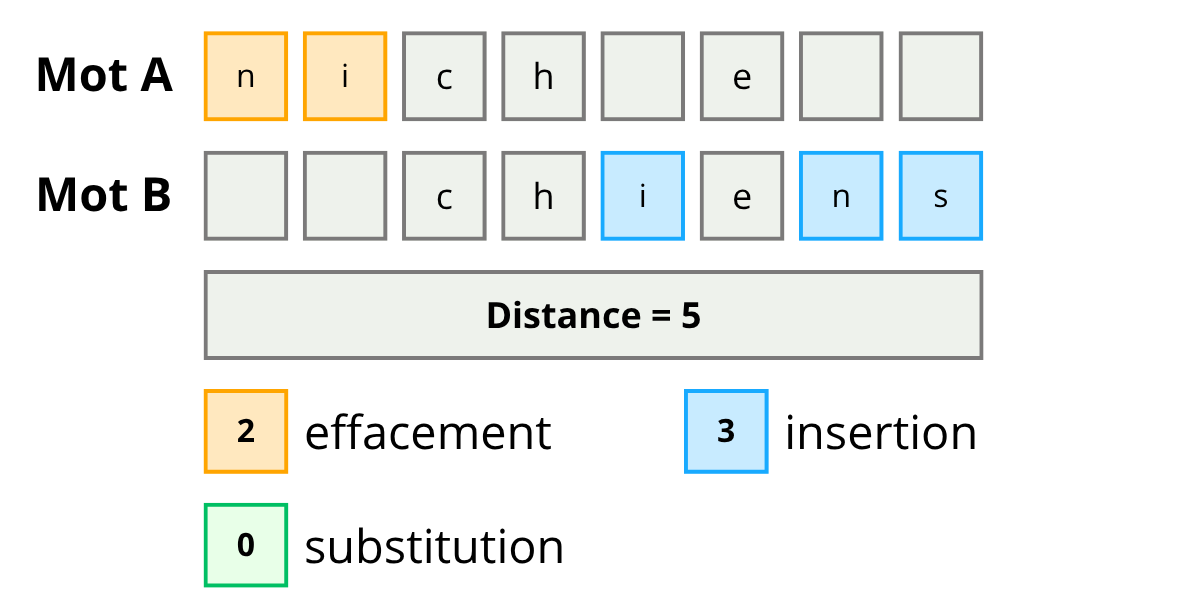
\includegraphics[width=0.9\textwidth]{images/levenshtein.png}
	\end{center}
	\textbf{Complexité : }  $\mathcal{O}(n \times m)$ (où n et m sont les longueurs des chaînes de caractères)
\end{frame}

\begin{frame}{Distance de Damerau-Levenshtein}
	\vspace*{-0.3cm}
	\textbf{Objectif : }identique à la distance de Levenshtein, mais avec l'ajout de la possibilité d'échanger deux caractères adjacents.
	\begin{center}
		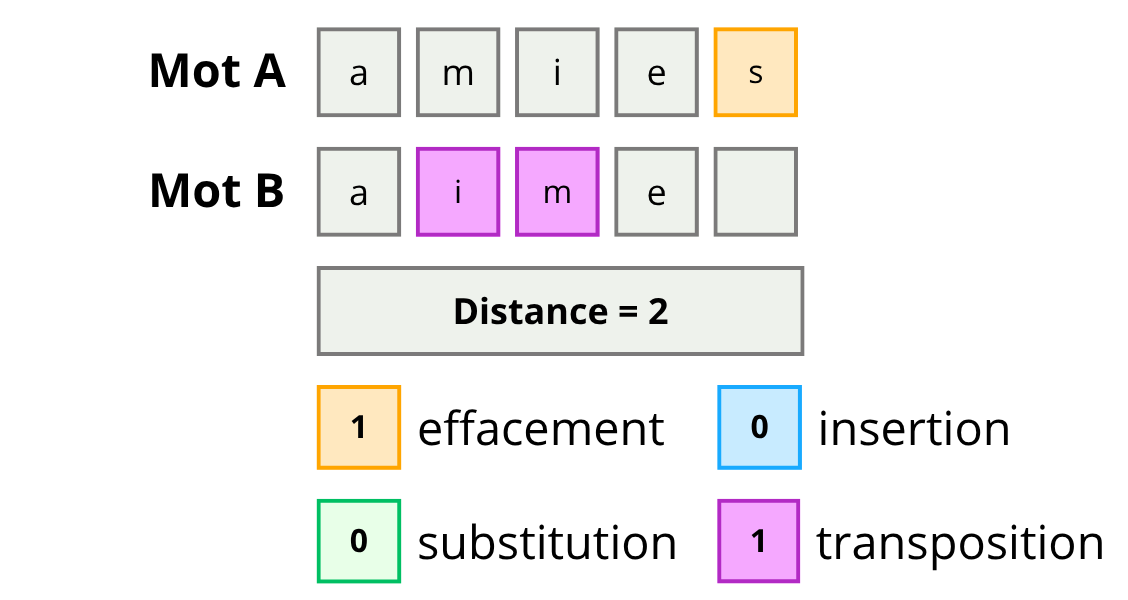
\includegraphics[width=0.9\textwidth]{images/damerau-levenshtein.png}
	\end{center}
	\textbf{Complexité : }  $\mathcal{O}(n \times m)$ (où n et m sont les longueurs des chaînes de caractères)
\end{frame}

\begin{frame}{Distance de Hamming}
	\begin{columns}
		\column{0.5\textwidth}
		Compter le nombre de positions où les caractères diffèrent.
		\column{0.5\textwidth}
		Utilisable que pour des mots de même longueur.
	\end{columns}
	\begin{center}
		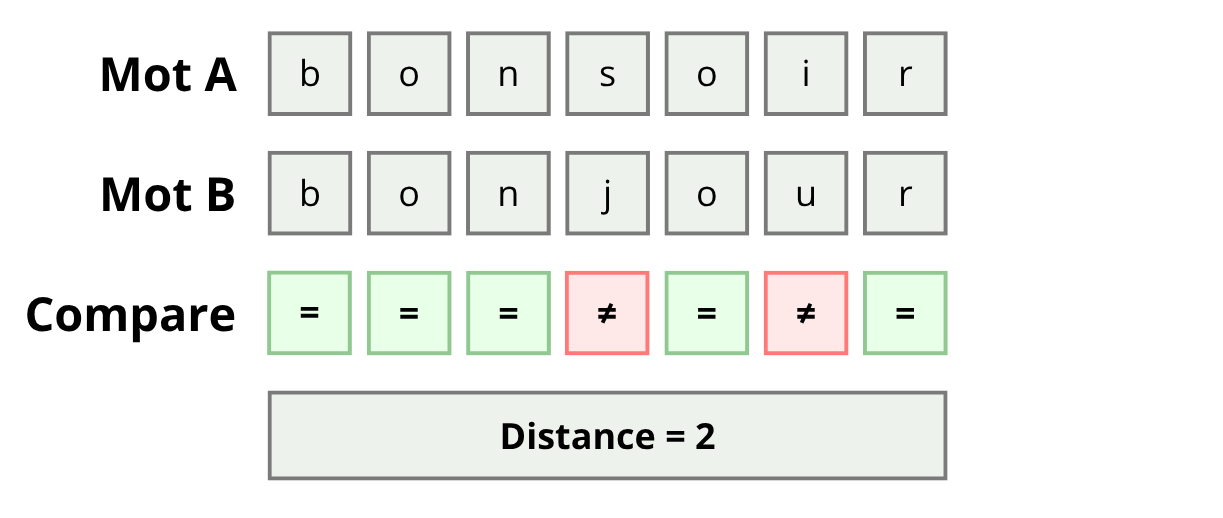
\includegraphics[width=0.9\textwidth]{images/hamming.png}
	\end{center}
	\textbf{Complexité : }  $\mathcal{O}(n)$ (où n est la longueur des chaînes de caractères)
\end{frame}

\section{Les chaînes de Markov}
% Un algorithme de calcul de distance permet de mesurer la similarité et/ou la dif-
% férence entre deux objets tels que du texte, des vecteurs, des chaînes de caractères.
% On utilise ces algorithmes de calcul principalement pour la correction d’orthographe,
% le traitement de texte, les alignements de séquences ADN ou encore pour la recherche
% d’information


\begin{frame}{Définition d'une chaîne de Markov}
	\begin{itemize}
		\item \textbf{Chaîne de Markov} : Modèle mathématique représentant un système de probabilité. Les probabilités de passer d'un état à un autre dépendent entièrement de l'état actuel.
		\item \textbf{Etats} : Elements du système.
		\item \textbf{Transition} : Action de passer d'un état à un autre.
		\item \textbf{Matrice transition} : Table permettant de regrouper les transitions entre tous les états.
	\end{itemize}
	\begin{center}
		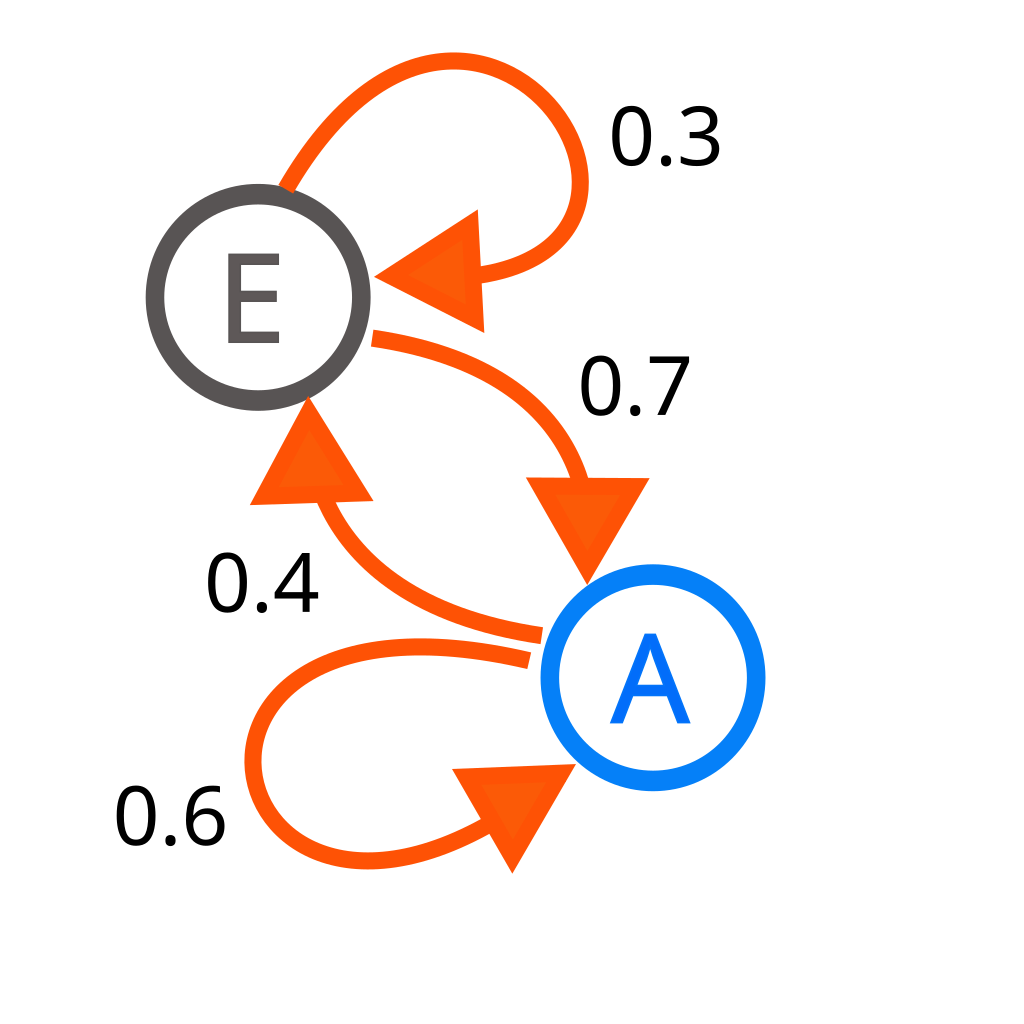
\includegraphics[width=0.38\textwidth]{images/def_markov.png}
		\vspace*{0.3cm}
	\end{center}

\end{frame}

\begin{frame}{Application}
	\vspace*{-0.3cm}
	Utilisation pour modélisation de processus aléatoires, analyse de séquences, de prédictions ou d'historiques de navigation.
	Analyse des historiques de navigation ainsi que les actions de l'utilisateur.

	\begin{center}
		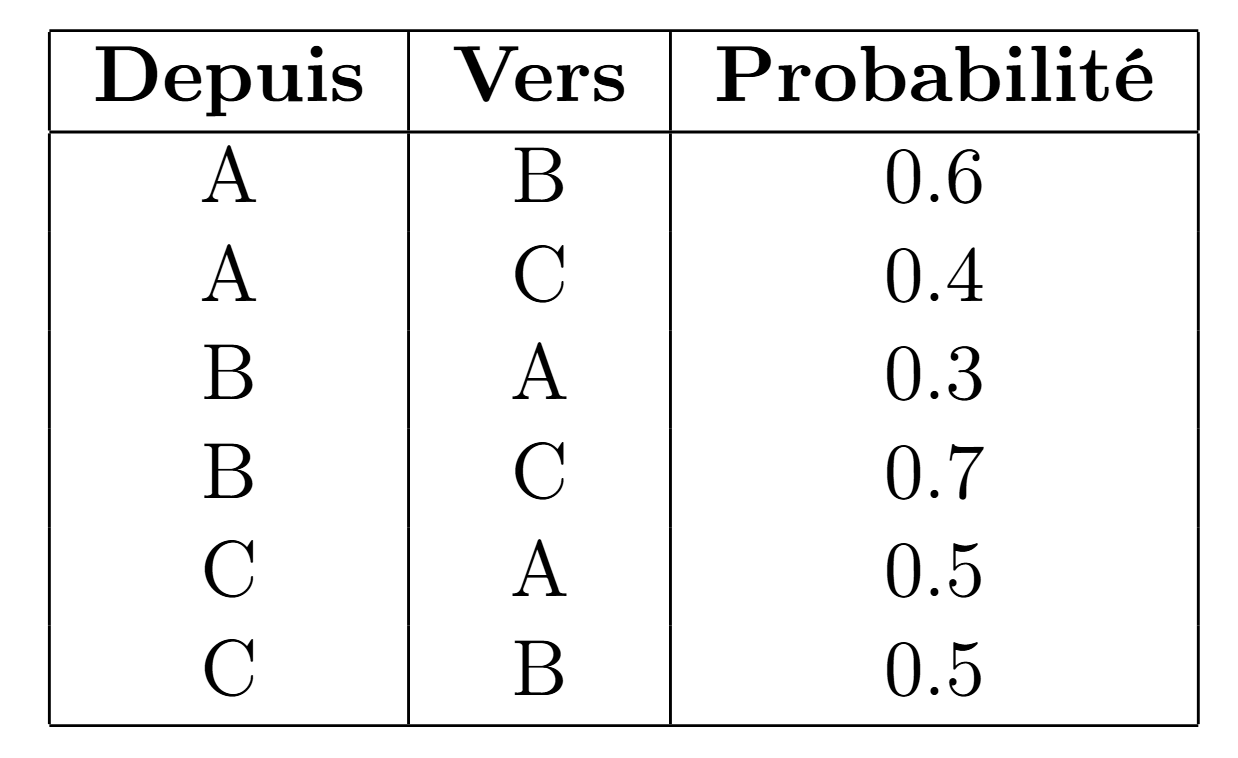
\includegraphics[width=0.6\textwidth]{images/tableau_proba_markov.png}
		\par
		\uline{Exemple transitions entre trois pages web A, B et C}
	\end{center}
\end{frame}

\begin{frame}{Matrice transition}
	Modélisation des transitions probables entre les étapes.
	\begin{itemize}
		\item Collecter les données
		\item Compter les transitions
		\item Calcul des probabilités
		\item Construction de la matrice
	\end{itemize}
	\begin{center}
		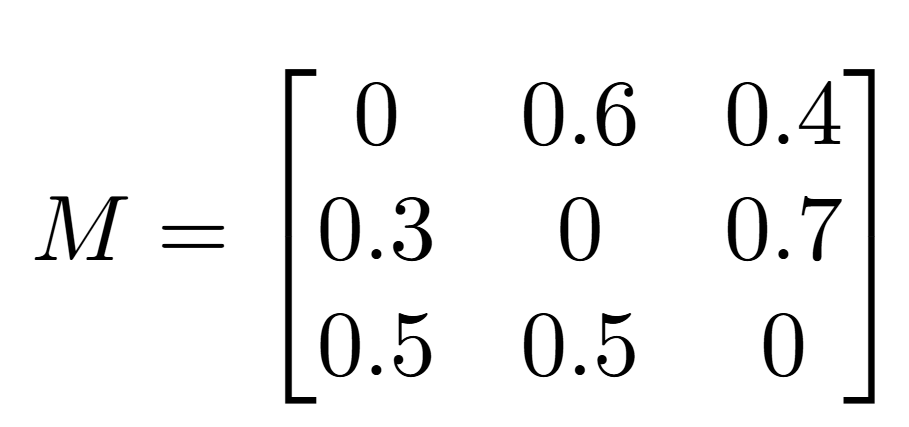
\includegraphics[width=0.6\textwidth]{images/matrice_transition.png}
		\par
		\uline{Résultat selon le tableau précédent}
	\end{center}
\end{frame}

\begin{frame}{Exemple complet}
	\vspace{-0.5cm}
	\centering
	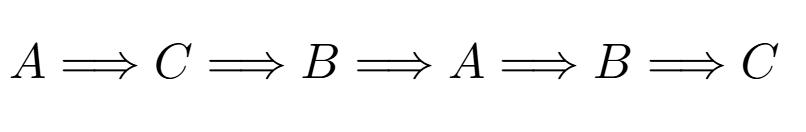
\includegraphics[width=0.8\textwidth]{images/transition_ex_markov.png}
	\vspace{1cm}
	\begin{columns}
		\column{0.6\textwidth}
		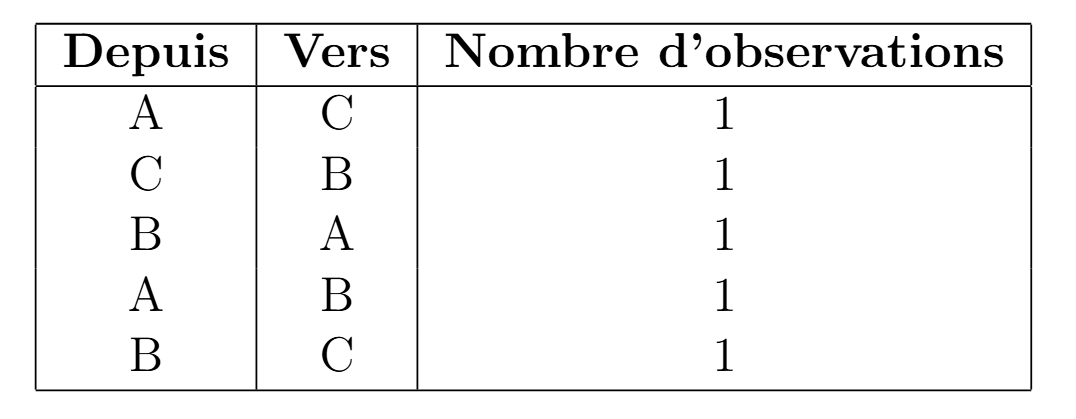
\includegraphics[width=\textwidth]{images/tableau_ex_markov.png}
		\column{0.4\textwidth}
		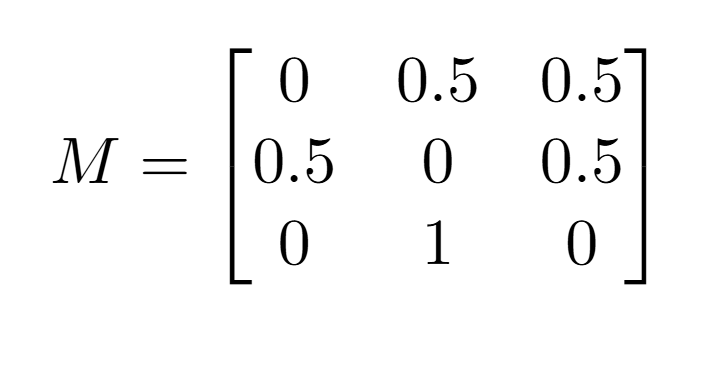
\includegraphics[width=\textwidth]{images/matrice_markov.png}
	\end{columns}
	\vspace{1cm}
	\textbf{Calcul probabilités} :  nombre de fois où la transition \(X\) vers \(Y\) est observée, puis de diviser par le total des transitions partant de l'état \(X\).
\end{frame}

\section{Notre outil de complétion semi-automatique}

\begin{frame}{Choix pour l'implémentation}
	\begin{columns}
		\column{0.5\textwidth}
		\textbf{Notre objectif~:}
		\begin{itemize}
			\item Reproduire un outil de complétion semi-automatique comme sur téléphone mais sur ordinateur
			\item Utilisable dans n'importe quel application
		\end{itemize}

		\column{0.5\textwidth}
		\begin{center}
			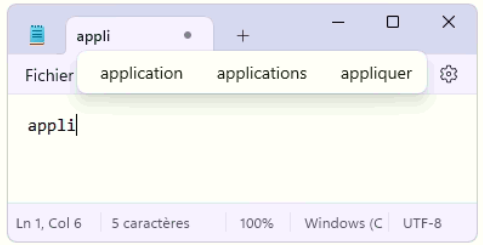
\includegraphics[width=\textwidth]{images/suggestion_windows.png}
			\uline{Outil de suggestion de mots sur Windows}
		\end{center}
	\end{columns}
	\vspace{0.5cm}
	\begin{columns}
		\column{0.5\textwidth}
		\textbf{Choix du langage~:}
		\begin{itemize}
			\item Apprendre un nouveau langage
			\item Langage de programmation moderne
			\item Conçu pour la performance
		\end{itemize}

		\column{0.5\textwidth}
		
\includegraphics[width=\textwidth]{images/rust.jpeg}
	\end{columns}
\end{frame}


\begin{frame}{Création du keylogger \& mouselogger}
	\vspace*{-0.5cm}
	\begin{columns}
		\column{0.5\textwidth}
		\begin{itemize}
			\item Détection des péréphériques
			\item Lecture des évenements
			\item Décodage avec le fichier \textbf{input-event-codes.h}
			\item Sauvegarde des évènements pour récupérer le mot tapé
		\end{itemize}
		\column{0.5\textwidth}
		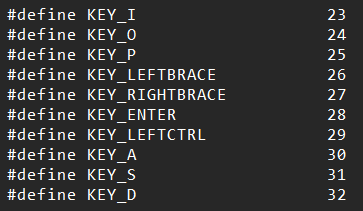
\includegraphics[width=\textwidth]{images/fichier_touche.png}
	\end{columns}
	\begin{center}
		\vspace*{-0.3cm}
		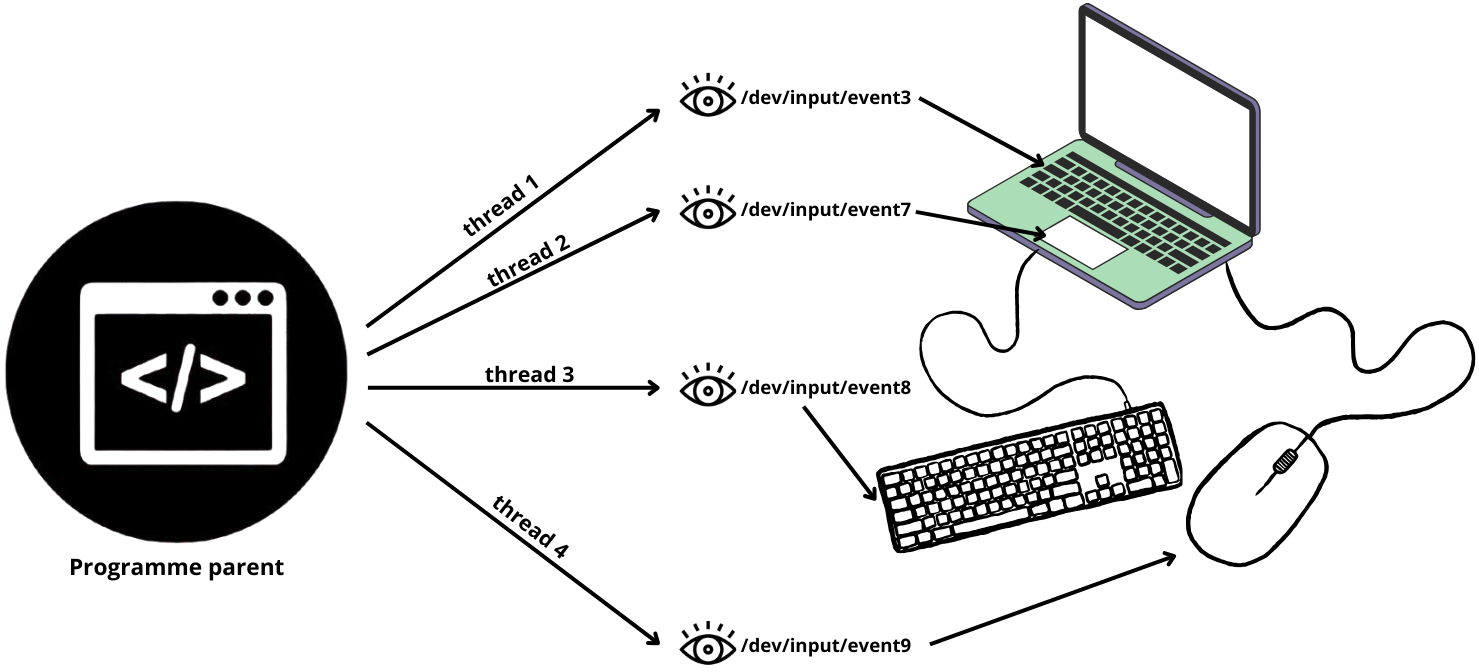
\includegraphics[width=\textwidth]{images/lecture-fichier-borderless.png}
	\end{center}

\end{frame}



\begin{frame}{Création du clavier virtuel}
	\textbf{Objectif~:} Ecrire le mot que l'utilisateur a choisi sur l'interface de l'application
	\begin{itemize}
		\item Traduction caractère → évènement clavier
		\item Envoi séquentiel des lettres du mot
		\item Suppression du mot précédent (retour arrière $n$ fois)
		\item Réécriture fluide et invisible
	\end{itemize}
\end{frame}


\begin{frame}{Algorithme de suggestion}
	Utilisation de la \textbf{distance de Levenshtein} pour la suggestion de mots

	\begin{itemize}
		\item Comparaison avec $\simeq$ 140 000 mots
		\item Sélection des mots les plus proches
	\end{itemize}

	\begin{block}{\alert{Résultats décevants}}
    \vspace{5pt}
		→ Suggestions peu pertinentes\\
		→ Nécessité d’ajouter des critères complémentaires
	\end{block}

	\textbf{Solutions apportées~:}
	\begin{itemize}
		\item Analyse des \textbf{préfixes}
		\item Pondération selon la \textbf{fréquence d'utilisation}
	\end{itemize}
\end{frame}

\begin{frame}{Algorithme de suggestion}
	\vspace*{-0.75cm}
	\begin{center}

		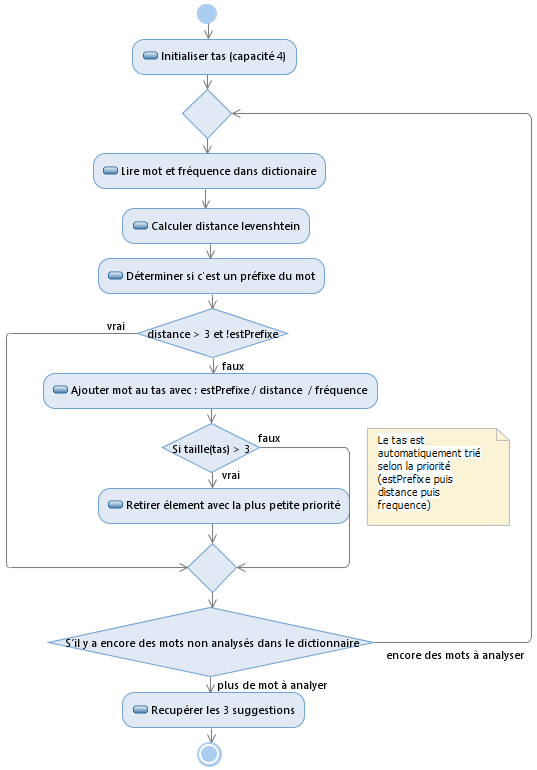
\includegraphics[height=0.98\textheight]{images/uml_diapo.png}
	\end{center}

\end{frame}




\begin{frame}{L'interface graphique}
	\begin{columns}
		\column{0.45\textwidth}
		\begin{itemize}
			\item Initialement, interface prévue en \textbf{Rust avec GTK}
			\item Problème : impossible de garder la fenêtre au premier plan constamment
			\item Solution : interface réalisée en \textbf{Python avec Tkinter}
			\item Communication entre Rust et Python via leur \textbf{entrée standard}
		\end{itemize}

		\column{0.50\textwidth}
		\centering
		\textbf{Interface finale :} \\
		
\includegraphics[width=\textwidth]{images/demo_interface.png}
	\end{columns}
\end{frame}


\begin{frame}{Installeur de l'application}
	\begin{itemize}
		\item Création d'un installeur pour l'application
		\item Utilisation d'un \textbf{Makefile}
		\item Pour
		      \begin{itemize}
			      \item Compiler le code
			      \item Attribuer les droits nécessaire
			      \item Créer le fichier \textbf{.desktop}
			      \item Déplacer le binaire
		      \end{itemize}
	\end{itemize}
	\begin{center}
		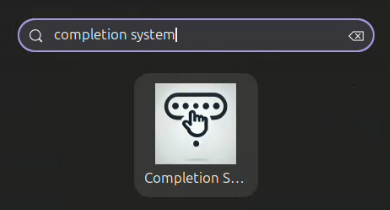
\includegraphics[width=0.5\textwidth]{images/application.png}
	\end{center}

\end{frame}

\section{Démonstration}% montrer la video

\section*{Questions}
\begin{frame}{Questions~?}
	\vspace*{-0.3cm}
	\begin{columns}
		\column{0.5\textwidth}
		\begin{center}
			
\includegraphics[width=0.6\textwidth]{images/logo_univ.png}
		\end{center}
		
		\column{0.5\textwidth}
		\begin{center}
			
\includegraphics[width=0.6\textwidth]{images/logo_CMI.png}
		\end{center}
		
	\end{columns}
	\vspace*{0.2cm}
	
	\centering
	\emph{Merci de votre attention~!}\\
	\vspace{0.6cm}
	\textbf{Avez-vous des questions~?}
	
\includegraphics[width=0.7\textwidth]{images/questions.png}
\end{frame}



\end{document}
